\documentclass[11pt,a4paper]{article}

% -----------------------------------------------------------------------------
% COMP9900 Project 18 final report (9900-F09C-ALMOND).
% Built from the client-review draft after client feedback on 1 August 2026.
% Remaining manual inserts before submission: the two screenshot figures.
% -----------------------------------------------------------------------------

\usepackage[T1]{fontenc}
\usepackage[utf8]{inputenc}
\usepackage{lmodern}
\usepackage[margin=2.3cm]{geometry}
\usepackage{microtype}
\usepackage{graphicx}
\usepackage{booktabs}
\usepackage{tabularx}
\usepackage{array}
\usepackage{xcolor}
\usepackage{enumitem}
\usepackage{listings}
\usepackage{hyperref}
\usepackage{fancyhdr}
\usepackage{tikz}
\usepackage{amssymb}
\usepackage{amsmath}
\usepackage{subcaption}

\usetikzlibrary{arrows.meta,positioning,shapes.geometric}

\definecolor{UNSWGold}{HTML}{FFD500}
\definecolor{Navy}{HTML}{0B1F3A}
\definecolor{Blue}{HTML}{2056A8}
\definecolor{PaleBlue}{HTML}{EDF4FF}
\definecolor{PaleGold}{HTML}{FFF8D8}
\definecolor{PaleGrey}{HTML}{F4F6F8}
\definecolor{DarkGrey}{HTML}{445064}

\hypersetup{
  colorlinks=true,
  linkcolor=Blue,
  citecolor=Blue,
  urlcolor=Blue,
  pdftitle={Project 18 Final Report},
  pdfauthor={9900-F09C-ALMOND}
}

\pagestyle{fancy}
\fancyhf{}
\lhead{COMP9900 Project 18}
\rhead{9900-F09C-ALMOND}
\cfoot{\thepage}
\setlength{\headheight}{14pt}

\setlist[itemize]{leftmargin=1.6em,itemsep=0.25em,topsep=0.4em}
\setlist[enumerate]{leftmargin=1.8em,itemsep=0.25em,topsep=0.4em}
\renewcommand{\arraystretch}{1.22}
\setcounter{tocdepth}{2}

\newcolumntype{Y}{>{\raggedright\arraybackslash}X}
\newcolumntype{L}[1]{>{\raggedright\arraybackslash}p{#1}}

\lstdefinestyle{terminal}{
  basicstyle=\ttfamily\small,
  backgroundcolor=\color{PaleGrey},
  frame=single,
  rulecolor=\color{DarkGrey!35},
  breaklines=true,
  columns=fullflexible,
  keepspaces=true,
  showstringspaces=false,
  xleftmargin=0.4em,
  xrightmargin=0.4em
}

\lstdefinestyle{prompt}{
  basicstyle=\ttfamily\footnotesize,
  backgroundcolor=\color{PaleGrey},
  frame=single,
  rulecolor=\color{DarkGrey!35},
  breaklines=true,
  breakindent=0pt,
  columns=fullflexible,
  keepspaces=true,
  showstringspaces=false,
  xleftmargin=0.4em,
  xrightmargin=0.4em
}

\newcommand{\stratone}{Strategy 1 (Propose and Verify)}
\newcommand{\strattwo}{Strategy 2 (Importance-Guided Infilling)}
\newcommand{\stratthree}{Strategy 3 (Concept-Guided Editing)}

\begin{document}

% =============================================================================
% Title page
% =============================================================================
\begin{titlepage}
  \thispagestyle{empty}

  \noindent\colorbox{UNSWGold}{\parbox[c][0.35cm][c]{\textwidth}{}}

  \vspace{1.3cm}
  {\Large\bfseries COMP9900 -- Information Technology Project\par}
  \vspace{0.5cm}
  {\huge\bfseries Project 18: Explainable LLMs for\\[0.2cm]
  Mental Health Support\par}
  \vspace{0.8cm}
  {\LARGE\color{Blue}\bfseries Project Report\par}

  \vspace{1.1cm}

  \begin{tabularx}{\textwidth}{@{}L{3.2cm}Y@{}}
    \textbf{Team} & 9900-F09C-ALMOND \\
    \textbf{Client} & Dr Thao Le \\
    \textbf{Submission date} & Week 10 Sunday, 9:00 pm \\
  \end{tabularx}

  \vspace{0.8cm}

  \begin{tabularx}{\textwidth}{@{}L{2.6cm}L{4.8cm}L{1.9cm}Y@{}}
    \toprule
    \textbf{Name} & \textbf{Email} & \textbf{Student ID} & \textbf{Role} \\
    \midrule
    Xi Shen & z5547747@ad.unsw.edu.au & z5547747 & Scrum Master, Backend \\
    Yidi Wu & z5561320@ad.unsw.edu.au & z5561320 & Backend \\
    Jiajun Wang & z5560250@ad.unsw.edu.au & z5560250 & Frontend \\
    Zijie Cai & z5529079@ad.unsw.edu.au & z5529079 & Backend \\
    Meitong Zhou & z5324147@ad.unsw.edu.au & z5324147 & Project Manager, Backend \\
    Jiaxin Liu & z5565763@ad.unsw.edu.au & z5565763 & Backend \\
    \bottomrule
  \end{tabularx}

  \vfill
\end{titlepage}

\pagenumbering{roman}
\tableofcontents
\newpage
\pagenumbering{arabic}

% =============================================================================
% Executive summary
% =============================================================================
\section*{Executive Summary}
\addcontentsline{toc}{section}{Executive Summary}

We built a local web tool for studying how a small open-source language model answers
emotional-reasoning questions from EmoBench \cite{sabour2024}. A user loads a scenario,
sees the model's answer, chooses a different answer (we call it the \emph{foil}), and
runs a search strategy that tries to change the model's answer to that foil by editing
only the scenario text. This follows the general idea of counterfactual explanations:
show the smallest change to the input that changes the output
\cite{wachter2018,miller2019}.

The system contains a simple word-level baseline and three main counterfactual
strategies: \stratone{}, \strattwo{}, and \stratthree{}. A common dev-40 run compared
all four on the same questions, foils, budget, frozen target model, and verification
path. The Baseline produced 13/40 primary review candidates, Strategy~1 produced
11/40, Strategy~2 produced 6/40, and Strategy~3 produced 5/40 plus six diagnostic
scenarios. These are within-set mechanical results, not population estimates or
human-valid rates.

This distinction between a \emph{mechanical flip} (there was a change in the model's
response), a \emph{human-valid explanation} (there is agreement that the edit is a
significant change), a \emph{diagnostic signal} (the model's response was affected by
the wording, spelling, or a hint of the answer that was leaked), and a legitimate
\texttt{not\_found} outcome (no flip within the budget) is critical since, according
to our tests in Sprint 2, a high flip rate may also imply larger, contradictory, or
even irrelevant edits.

In Sprint 3 we introduced a shared minimality test phase, a fluency test, developed a
discovery version for each strategy, refined the labels in the user interface, and
included accessibility options. This report describes the design that we have finally
come up with, provides the results of our measurement experiments, and presents
examples of provisionally acceptable, invalid, and diagnostic outcomes. It clearly
states what goals we have reached and what goals we have missed. Every flip presented
is treated as an illustration of model behavior in a fixed environment.

% =============================================================================
% 1. Installation manual
% =============================================================================
\section{Installation Manual}

The application is dockerised. Docker Compose builds and starts the backend (FastAPI)
and the frontend (React build served by nginx). Ollama stays on the host machine
because it manages the local language models; the project deliberately uses no paid
cloud API. The exact Python, Node, and package versions are pinned in the repository
(\texttt{backend/requirements.txt}, \texttt{frontend/package-lock.json}) and are listed
in the repository README, so the report only describes the steps to run.

\subsection{Prerequisites and Setup}

The machine needs Docker Desktop (or Docker Engine with Compose), Ollama, and the two
EmoBench data files (\texttt{EU.jsonl}, \texttt{EA.jsonl}), which are supplied
separately because the benchmark data is not committed to Git.

\begin{lstlisting}[style=terminal,language=bash]
# 1. Clone the repository and enter it
git clone https://github.com/unsw-cse-comp99-3900/capstone-project-26t2-9900-f09c-almond.git
cd capstone-project-26t2-9900-f09c-almond

# 2. Start Ollama on the host and pull the frozen local model
ollama pull llama3.2:3b

# 3. Place EU.jsonl and EA.jsonl in data/raw/

# 4. Build and start the application
docker compose up --build -d

# 5. Load the EmoBench data into SQLite (one-off)
docker compose exec backend python -m app.scripts.load_emobench \
  --input /data/raw/EU.jsonl
docker compose exec backend python -m app.scripts.load_emobench \
  --input /data/raw/EA.jsonl
\end{lstlisting}

The frontend is then available at \url{http://localhost:5173} and the backend API
documentation at \url{http://localhost:8000/docs}. \texttt{docker compose down} stops
the application. The named SQLite volume preserves imported scenarios,
target-prediction cache entries, experiment-run metadata, and job checkpoints across
container restarts. Completed counterfactual payloads, metrics, and batch-comparison
results are currently retained in process memory and must be rerun after a backend
restart. The README also includes instructions for developing without Docker using
Python 3.11 virtualenv and \texttt{npm run dev}.

\subsection{Environment Variables and Secrets}

No API key or cloud services are required to use this project. All configuration is
easy environment variables with reasonable defaults defined in
\texttt{docker-compose.yml} (or else you may use \texttt{backend/.env.example} if
running manually). Table~\ref{tab:env} describes environment variables that can be
modified.

\begin{table}[htbp]
\centering
\small
\begin{tabularx}{\textwidth}{@{}L{4.2cm}Y L{3.9cm}@{}}
\toprule
\textbf{Variable} & \textbf{Purpose} & \textbf{Release setting} \\
\midrule
\texttt{USE\_MOCK\_LLM} & Deterministic mock mode or real local Ollama & \texttt{false} for real runs \\
\texttt{REPO\_BACKEND} & Memory or SQLite persistence & \texttt{sqlite} \\
\texttt{DATABASE\_URL} & SQLite location & Docker volume path \\
\texttt{OLLAMA\_BASE\_URL} & Local model endpoint & \texttt{http://host.docker.internal:11434} \\
\texttt{DEFAULT\_MODEL} & Frozen target model & \texttt{llama3.2:3b} for the current evaluation setup \\
\texttt{VITE\_API\_BASE\_URL} & Frontend-to-backend endpoint & \texttt{http://localhost:8000}, configured in \texttt{frontend/.env.example} \\
\bottomrule
\end{tabularx}
\caption{Environment configuration.}
\label{tab:env}
\end{table}

\subsection{Clean-Machine Verification}

We verified the dockerised installation on a Windows 11 machine with Docker Desktop by
following exactly the steps above from a clean checkout: both images built, both
containers started, the backend health endpoint reported real (non-mock) mode, both
EmoBench files loaded into SQLite, one real prediction ran through the containerised
backend against the host Ollama model, and the containers were restarted without
losing the SQLite-backed scenarios, target-prediction cache entries, experiment-run
metadata, or job checkpoints. Completed counterfactual payloads, metrics, and
batch-comparison results were not treated as restart-persistent. The tested Docker,
Ollama, and model digest values are recorded in the repository README.

% =============================================================================
% 2. Architecture
% =============================================================================
\section{System Architecture Diagram}

Figure~\ref{fig:architecture} presents the architecture developed. Each strategy search has one quality pipeline
that is shared, meaning minimality, fluency, risk labels, and metrics are computed the
same for all results.

\begin{figure}[htbp]
\centering
\resizebox{0.98\textwidth}{!}{%
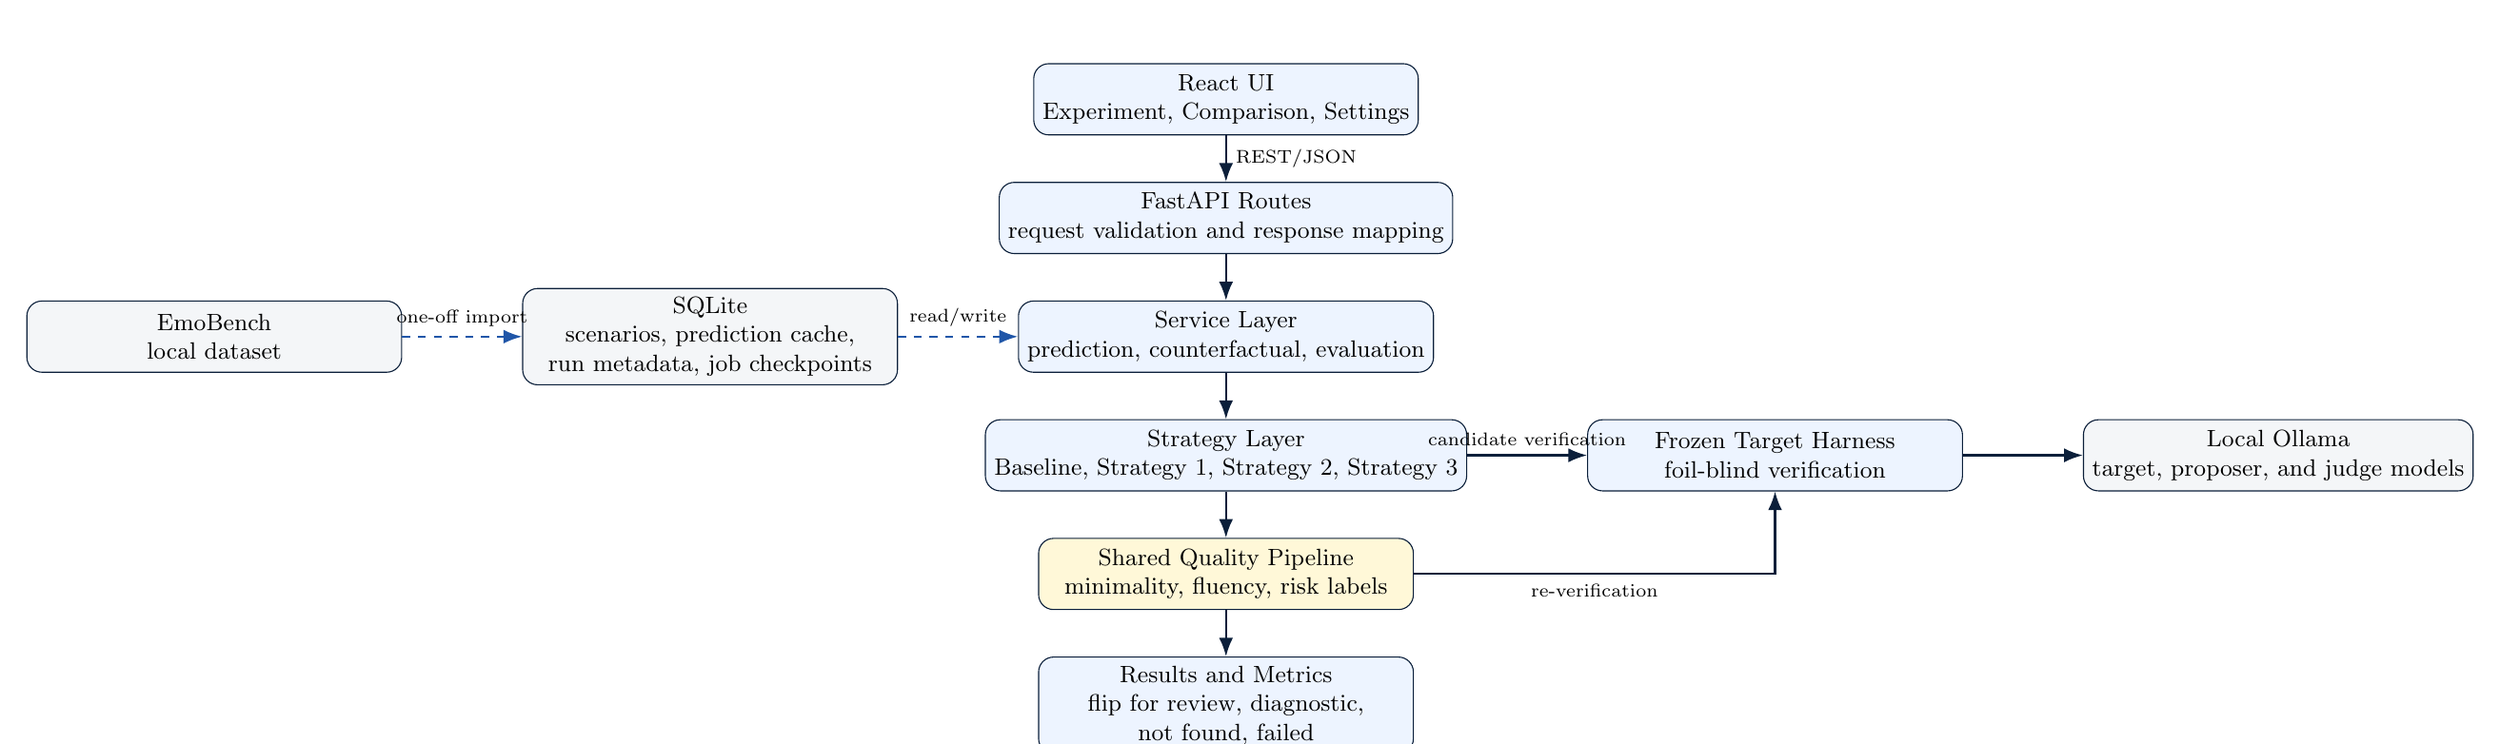
\begin{tikzpicture}[
  node distance=0.62cm and 1.6cm,
  block/.style={
    draw=Navy,
    rounded corners=2mm,
    fill=PaleBlue,
    align=center,
    minimum width=5.0cm,
    minimum height=0.95cm,
    font=\small
  },
  quality/.style={
    block,
    fill=PaleGold
  },
  source/.style={
    block,
    fill=PaleGrey
  },
  flow/.style={-{Latex[length=2.5mm]},thick,draw=Navy},
  dataflow/.style={-{Latex[length=2.5mm]},thick,draw=Blue,dashed}
]
  \node[block] (ui) {React UI\\Experiment, Comparison, Settings};
  \node[block, below=of ui] (api) {FastAPI Routes\\request validation and response mapping};
  \node[block, below=of api] (services) {Service Layer\\prediction, counterfactual, evaluation};
  \node[block, below=of services] (strategies) {Strategy Layer\\Baseline, Strategy 1, Strategy 2, Strategy 3};
  \node[quality, below=of strategies] (quality) {Shared Quality Pipeline\\minimality, fluency, risk labels};
  \node[block, below=of quality] (results) {Results and Metrics\\flip for review, diagnostic,\\not found, failed};

  \node[source, left=of services] (sqlite) {SQLite\\scenarios, prediction cache,\\run metadata, job checkpoints};
  \node[source, left=of sqlite] (emobench) {EmoBench\\local dataset};
  \node[block, right=of strategies] (target) {Frozen Target Harness\\foil-blind verification};
  \node[source, right=of target] (ollama) {Local Ollama\\target, proposer, and judge models};

  \draw[flow] (ui) -- node[right,font=\scriptsize]{REST/JSON} (api);
  \draw[flow] (api) -- (services);
  \draw[flow] (services) -- (strategies);
  \draw[flow] (strategies) -- (quality);
  \draw[flow] (quality) -- (results);
  \draw[dataflow] (emobench) -- node[above,font=\scriptsize]{one-off import} (sqlite);
  \draw[dataflow] (sqlite) -- node[above,font=\scriptsize]{read/write} (services);
  \draw[flow] (strategies) -- node[above,font=\scriptsize]{candidate verification} (target);
  \draw[flow] (quality) -| node[near start,below,font=\scriptsize]{re-verification} (target);
  \draw[flow] (target) -- (ollama);
\end{tikzpicture}%
}
\caption{Final architecture. The Strategy Layer contains the word-level Baseline and
the three main strategies; all of them verify candidates only through the Frozen
Target Harness.}
\label{fig:architecture}
\end{figure}

\subsection{Major Components and Data Flow}

\begin{enumerate}
  \item The user selects an EmoBench scenario and the local model in the React
  interface.
  \item The backend asks the frozen target harness for the original answer. The target
  prompt is stateless and deterministic, and it never contains the foil.
  \item The user selects a foil and one strategy (Baseline, Strategy 1, Strategy 2, or
  Strategy 3, each with a strict or discovery variant where available).
  \item The strategy proposes scenario edits in its own way. Only the frozen target
  decides whether a candidate reaches the foil.
  \item The process of a successful candidate is followed by minimality, fluency
  scoring, and risk labelling before metric recording and display.
  \item A search which exhausts its budget without flipping becomes
  \texttt{not\_found}. It is not converted to an error, and nothing is made up as an
  explanation for it.
\end{enumerate}

Since all strategies have the same target function, target prompt version, success
criterion, budget, and metric definitions within a controlled run, the only thing that
could distinguish different strategies is their search methods.

% =============================================================================
% 3. Design justifications
% =============================================================================
\section{Design Justifications}

We designed the system to support a controlled comparison of counterfactual search
strategies rather than to maximise the number of answer flips. For the completion of this objective,
a frozen target user interface was needed for all strategies
(Chapter~\ref{sec:harness}), as well as strategy groups with different search
hypotheses (Chapter~\ref{sec:strategies}). Also, shared quality phases were needed,
which are unable to classify a flip independently as a valid explanation
(Chapter~\ref{sec:quality}). The numerical parameters used in this chapter (0.60
fraction changed, 0.75 fluency, three flips limitation and overbroad span rule)
are the choices made in implementation, rather than calibrated constants. Each
design choice was driven by experiments and feedback of the client and tutor.
Table~\ref{tab:evolution} shows a summary of key changes during the three sprints.

\begin{table}[htbp]
\centering
\small
\begin{tabularx}{\textwidth}{@{}L{1.7cm}Y Y Y@{}}
\toprule
\textbf{Stage} & \textbf{Goal at the start} & \textbf{Problem observed} & \textbf{Change made} \\
\midrule
Sprint 1 & Develop the MVP (minimal viable product) end-to-end locally and the first mechanical strategy. & The results from the strategies cannot be compared in a reliable way if the target prompts or success tests are different. The exhaustive search requires a clearly defined result. & Route every prediction through the frozen target harness and give all strategies the same interface. \\
Sprint 2 & Three core strategies: persistence and fair comparison & Testing more candidates produced more flips, but some edits were too large, contradicted the scenario, read unnaturally, or exposed the answer. & We added event grounding, safety checks, diagnostic labels, a reproducible comparison process, and an initial human validity review. \\
Sprint 3 & Improve the usefulness of the explanations and make the interface easier to use. & Fixed word limits rejected some useful edits, and flip rate alone could not tell meaningful changes from model sensitivity. & Let each strategy search more broadly within the safety limits, then run the shared minimality and fluency checks and keep review candidates separate from diagnostic findings. \\
\bottomrule
\end{tabularx}
\caption{Design changes from Sprint 1 to Sprint 3.}
\label{tab:evolution}
\end{table}

\subsection{Terminology and Outcome Categories}
\label{sec:terms}

We use the following terms throughout the report.

\begin{itemize}
  \item \textbf{Foil.} The foil is the alternative answer that the user wants the
  model to give. A search strategy may use the foil, whereas the target model never
  sees it.
  \item \textbf{Mechanical flip.} The frozen target model produces a mechanical flip
  when its answer after an edit matches the foil exactly. This result establishes
  that the answer changed. It does not establish that the edit provides a sound
  explanation.
  \item \textbf{Minimality.} Minimality refers to the size of the edit. We measure edit
  size by word-level edit distance: the number of single-word insertions, deletions,
  and replacements needed to convert one scenario to another. Additionally, we
  measure the changed-word fraction as a ratio of the above number to the scenario
  length in words. Smaller edits are easier to analyze and read.
  \item \textbf{Fluency.} Fluency measures how naturally the edited text reads in
  English. For this purpose, we utilize a local judge model
  (Section~\ref{sec:quality}) and take its score as a proxy, not a proof.
  \item \textbf{Semantic validity.} We define semantic validity as a change to some
  meaningful aspect of the event, outcome, relation, or behavior in the scenario. The
  examples of invalid flips include copying of the answer into the text, word
  replacement with a synonym, and contradiction to the story context. Our code
  highlights clear examples, and human judges resolve other flips manually through
  labeling as Good, Acceptable, or Invalid with reason codes provided.
  \item \textbf{Diagnostic finding.} Diagnostic finding refers to a verified flip
  associated with a risk flag, such as near-synonym substitution or answer leakage.
  We preserve the finding as suspected sensitivity evidence but do not present it as
  an explanation.
  \item \textbf{Budget.} The budget determines the maximum number of checks of the
  target model that a strategy can make on one scenario. Search and post-processing
  have their own budget limits. We record every check so that the reported costs
  include both stages.
\end{itemize}

These labels are hierarchical since a mechanical flip is required for counterfactual
explanation but is insufficient by itself. The automated classifier places each run
into precisely one of four categories: mechanical flip (requires review), diagnostic
observation, not found, and failed. The results of the entire process are reported using
the four categories in section~4 (Figure~\ref{fig:taxonomy}). The names Good,
Acceptable and Invalid refer to the external blinded review methodology discussed in
Section~\ref{sec:review}. The automated pipeline may flag flips as requiring review.
Even when reviewing one such run fully, all four retained review candidates were
mechanically verified, fluent, and moderate size but all were deemed Invalid
(Section~\ref{sec:review}). This illustrates the separation of automatic categories
from human judgment.

\begin{figure}[htbp]
\centering
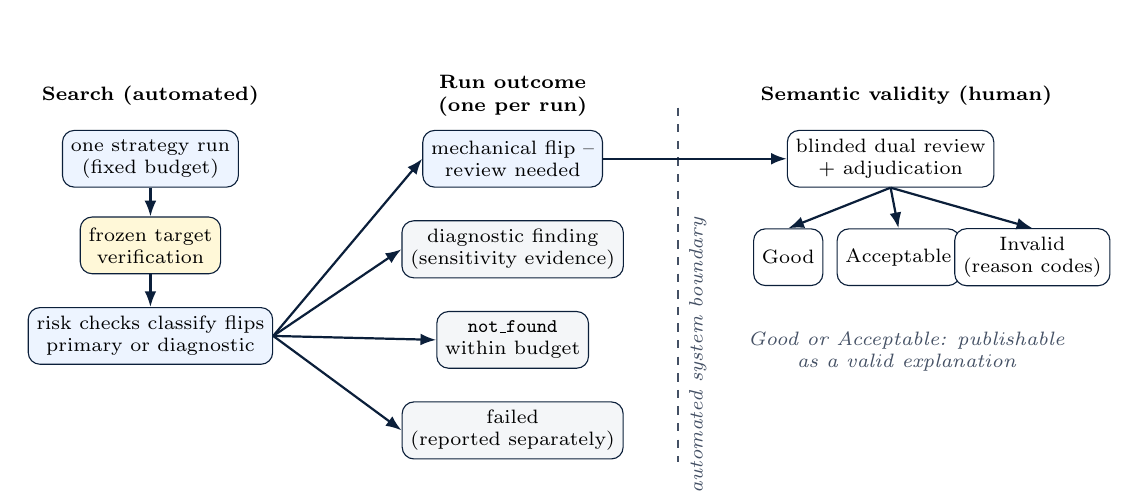
\begin{tikzpicture}[
  sbox/.style={draw=Navy,rounded corners=1.5mm,fill=PaleBlue,align=center,
    font=\scriptsize,minimum height=0.72cm,inner sep=3pt},
  tbox/.style={sbox,fill=PaleGold},
  gbox/.style={sbox,fill=PaleGrey},
  wbox/.style={sbox,fill=white},
  hdr/.style={font=\scriptsize\bfseries,align=center},
  note/.style={font=\scriptsize\itshape,text=DarkGrey,align=center},
  arr/.style={-{Latex[length=2mm]},thick,draw=Navy}
]
  % column headers
  \node[hdr] at (0,2.9)   {Search (automated)};
  \node[hdr] at (4.6,2.9) {Run outcome\\(one per run)};
  \node[hdr] at (9.6,2.9) {Semantic validity (human)};

  % column 1: search
  \node[sbox] (run)    at (0,2.1)   {one strategy run\\(fixed budget)};
  \node[tbox] (verify) at (0,1.0)   {frozen target\\verification};
  \node[sbox] (risk)   at (0,-0.15) {risk checks classify flips\\primary or diagnostic};
  \draw[arr] (run)--(verify);
  \draw[arr] (verify)--(risk);

  % column 2: one outcome category per run
  \node[sbox] (mech) at (4.6,2.1)   {mechanical flip --\\review needed};
  \node[gbox] (diag) at (4.6,0.95)  {diagnostic finding\\(sensitivity evidence)};
  \node[gbox] (nf)   at (4.6,-0.2)  {\texttt{not\_found}\\within budget};
  \node[gbox] (fail) at (4.6,-1.35) {failed\\(reported separately)};
  \draw[arr] (risk.east)--(mech.west);
  \draw[arr] (risk.east)--(diag.west);
  \draw[arr] (risk.east)--(nf.west);
  \draw[arr] (risk.east)--(fail.west);

  % boundary between automated system and external human review
  \draw[dashed,thick,draw=DarkGrey] (6.7,2.75) -- (6.7,-1.75);
  \node[note,rotate=90] at (6.95,-0.4) {automated system boundary};

  % column 3: external human review
  \node[wbox] (review) at (9.4,2.1) {blinded dual review\\+ adjudication};
  \draw[arr] (mech.east)--(review.west);
  \node[wbox] (good) at (8.1,0.85)  {Good};
  \node[wbox] (acc)  at (9.5,0.85)  {Acceptable};
  \node[wbox] (inv)  at (11.2,0.85) {Invalid\\(reason codes)};
  \draw[arr] (review.south)--(good.north);
  \draw[arr] (review.south)--(acc.north);
  \draw[arr] (review.south)--(inv.north);
  \node[note] at (9.6,-0.35) {Good or Acceptable: publishable\\as a valid explanation};
\end{tikzpicture}
\caption{Outcome taxonomy. Blue boxes are automated processing, the yellow box is
frozen-target verification, and grey boxes are terminal recorded outcomes; each run
receives exactly one outcome category (middle column). Everything right of the
dashed line is the external blinded human review: the Good, Acceptable, and Invalid
labels are never generated by the software itself.}
\label{fig:taxonomy}
\end{figure}

\subsection{Frozen Target Harness}
\label{sec:harness}

The system searches for counterfactual edits to a fixed black-box model. Every
strategy uses the same target prompt, decoding configuration, answer parser, and
cache contract. If strategies could change the target prompt, an observed difference
could arise from either the prompt or the edit. Appendix~\ref{app:prompts} provides
the full target prompt. We classify an edit as a flip when
\texttt{prediction.answer == foil}.

We also considered allowing each strategy to tune its own target prompt. Although
this alternative approach would help to achieve higher flip rates for each
individual case, it would be solving a different problem. The experiment
compares the effectiveness of \emph{search procedures}, not prompts that make the
model the most malleable. Freezing the target prompt, decoder configuration,
parser, and cache helps to avoid confounding on the target side, but there is still
some variation. The proposer is sampling at temperature 0.7 and cannot be
repeated byte-for-byte. Thus, Section~4 provides paired comparisons of same-job
runs (Sections~\ref{sec:s1results} and~\ref{sec:s3results}), and uses
the single-run runtime table (Section~\ref{sec:runtime}) to illustrate the magnitude
of costs.

\subsection{Strategy Families}
\label{sec:strategies}

The four implemented families cover progressively more structured units of change: a
fixed word list, a free event-level rewrite, an importance-guided span infill, and a
single grounded concept intervention. The comparison therefore tests different search
hypotheses rather than variants of one prompt. On the client's request, the report
applies the names Strategies 1--3 and Baseline to refer to these strategies.
Appendix~\ref{app:mapping} maps these terms to the corresponding identifiers in the
code and in the experiment metadata. Figure~\ref{fig:flows} illustrates the search
procedures for all these strategies.

The actual scope is different from the proposed scope, which included six
strategy families (identifier S1 to S6). This report covers four strategy families:
S1 (Baseline), S2 (Strategy~1), S4 (Strategy~2), and S6 (Strategy~3). Each main
family contains a strict variant and a discovery variant. We have not yet developed
the control code strategy family (S3) or the population-based search strategy family
(S5), and neither has been used for any results in this report. Both are future
work (Table~\ref{tab:future}).

\paragraph{Baseline: word-level greedy search.}
The Baseline performs simple word and phrase replacements on a predetermined list,
and checks every attempt. Since the candidates stem from this predetermined list,
the method does not employ any LLM to generate new samples. Consequently, the
search is transparent and cheap, making the approach an effective baseline, but the
changes made cannot represent an event as a whole.

\paragraph{\stratone{}.}
Local proposer LLM goes through the scenario, choices and foil and produces full
rewrites which change one event, outcome, relationship or observable behavior.
Deterministic guards filter out candidates which violate the structure, give away
the answer, or exceed the maximum edit size. The frozen target verifies all of
remaining candidates. In the Sprint 2 version (\emph{strict}), the goal is to change
around three words, while six changes are allowed. In Sprint 3 \emph{discovery}
version, the fixed number of changes is removed but the safety fraction of changes
is set to 0.60. The version retains up to three different verified flips and
sends the best candidate into the quality pipeline. The design builds upon the
zero-shot LLM counterfactual proposal in \cite{bhattacharjee2024}, keeping the
target model and verification constant.

\paragraph{\strattwo{}.}
This approach first determines the importance of each text span by temporarily
masking (occluding) one span at a time, querying the frozen target for the change in confidence in
the answer, and ranking spans in order of importance. In case of missing confidence
values, the strategy runs the answer-change heuristic and returns the coverage that
it achieves. The LLM proposer then modifies content in the top-ranked spans, and
the frozen target verifies each modification. This is an adaptation of the importance-guided
contrastive editing method \cite{ross2021} to a black-box setting. The discovery
approach splits its budget into probes of importance and checks of candidates.
It probes several top-ranked spans and mask widths, and records diagnostic
candidates separately. Both approaches have been implemented and unit tested, and both
of them passed a real model smoke test. The Discovery variant was included in the
common dev-40 matrix, but a paired strict-versus-Discovery evaluation was not
performed (Section~4).

\paragraph{\stratthree{}.}
This strategy changes one situational concept, such as time, place, relationship,
urgency, or outcome. The proposer LLM identifies an exact span and supplies a
replacement. Our code checks that the span occurs once before applying the edit,
preventing the LLM from rewriting the full story. The method draws on concept-level
counterfactual work \cite{gat2024}. We describe it as \emph{causal-inspired} because
changing one concept and observing the model constitutes an intervention on the
text. The intervention does not establish real-world causality. The discovery
variant adds an outcome concept class and permits a coherent multi-word replacement
span. It classifies an overbroad span (at least 12 tokens and more than half of the
scenario) as a diagnostic finding.

\paragraph{Strict and discovery variants.}
The variation split represents a design trade-off rather than a progression of
software versions. Sprint~2 demonstrated that using a word limit on a per-strategy
basis was premature for minimisation. It discarded sensible event-level
candidates prior to evaluation by the shared minimiser (Table~\ref{tab:prelim}).
Therefore, the discovery variants explore a wider space with bounded budgets and
safety caps, where shrinking, scoring, and classification is left up to the shared
pipeline. As part of the dev-40 pair run, we observed widened exploration along
with higher raw edit counts and greater invocation counts
(Table~\ref{tab:s1}). The strict variants retain their default status and serve as
the baseline for the change in Sprint~3.

\begin{figure}[htbp]
\centering
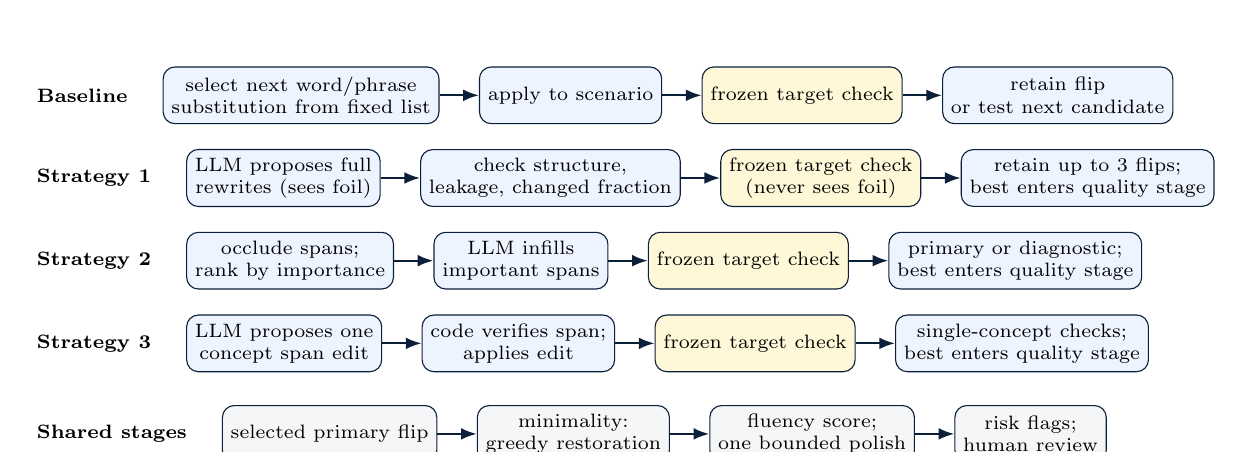
\begin{tikzpicture}[
  sbox/.style={draw=Navy,rounded corners=1.5mm,fill=PaleBlue,align=center,
    font=\scriptsize,minimum height=0.72cm,inner sep=3pt},
  tbox/.style={sbox,fill=PaleGold},
  lbl/.style={font=\scriptsize\bfseries,anchor=west},
  arr/.style={-{Latex[length=2mm]},thick,draw=Navy}
]
  % Baseline
  \node[lbl] (l0) at (0,0) {Baseline};
  \node[sbox,right=0.32cm of l0] (b1) {select next word/phrase\\substitution from fixed list};
  \node[sbox,right=0.5cm of b1] (b2) {apply to scenario};
  \node[tbox,right=0.5cm of b2] (b3) {frozen target check};
  \node[sbox,right=0.5cm of b3] (b4) {retain flip\\or test next candidate};
  \draw[arr] (b1)--(b2); \draw[arr] (b2)--(b3); \draw[arr] (b3)--(b4);

  % S1
  \node[lbl,below=1.05cm of l0.west,anchor=west] (l1) {Strategy 1};
  \node[sbox,right=0.32cm of l1] (s11) {LLM proposes full\\rewrites (sees foil)};
  \node[sbox,right=0.5cm of s11] (s12) {check structure,\\leakage, changed fraction};
  \node[tbox,right=0.5cm of s12] (s13) {frozen target check\\(never sees foil)};
  \node[sbox,right=0.5cm of s13] (s14) {retain up to 3 flips;\\best enters quality stage};
  \draw[arr] (s11)--(s12); \draw[arr] (s12)--(s13); \draw[arr] (s13)--(s14);

  % S2
  \node[lbl,below=1.05cm of l1.west,anchor=west] (l2) {Strategy 2};
  \node[sbox,right=0.32cm of l2] (s21) {occlude spans;\\rank by importance};
  \node[sbox,right=0.5cm of s21] (s22) {LLM infills\\important spans};
  \node[tbox,right=0.5cm of s22] (s23) {frozen target check};
  \node[sbox,right=0.5cm of s23] (s24) {primary or diagnostic;\\best enters quality stage};
  \draw[arr] (s21)--(s22); \draw[arr] (s22)--(s23); \draw[arr] (s23)--(s24);

  % S3
  \node[lbl,below=1.05cm of l2.west,anchor=west] (l3) {Strategy 3};
  \node[sbox,right=0.32cm of l3] (s31) {LLM proposes one\\concept span edit};
  \node[sbox,right=0.5cm of s31] (s32) {code verifies span;\\applies edit};
  \node[tbox,right=0.5cm of s32] (s33) {frozen target check};
  \node[sbox,right=0.5cm of s33] (s34) {single-concept checks;\\best enters quality stage};
  \draw[arr] (s31)--(s32); \draw[arr] (s32)--(s33); \draw[arr] (s33)--(s34);

  % Shared pipeline
  \node[lbl,below=1.15cm of l3.west,anchor=west] (l4) {Shared stages};
  \node[sbox,right=0.32cm of l4,fill=PaleGrey] (q1) {selected primary flip};
  \node[sbox,right=0.5cm of q1,fill=PaleGrey] (q2) {minimality:\\greedy restoration};
  \node[sbox,right=0.5cm of q2,fill=PaleGrey] (q3) {fluency score;\\one bounded polish};
  \node[sbox,right=0.5cm of q3,fill=PaleGrey] (q4) {risk flags;\\human review};
  \draw[arr] (q1)--(q2); \draw[arr] (q2)--(q3); \draw[arr] (q3)--(q4);
\end{tikzpicture}
\caption{Search process for each strategy. Yellow boxes mark frozen target checks,
which are the only mechanism available for testing a candidate. The selected primary
flip then passes through the shared quality stages in the bottom row, while
diagnostic flips are retained separately as sensitivity evidence. Each shared stage
that changes the scenario re-verifies the flip through the same frozen target;
stages that only score, classify, or record make no further target call.}
\label{fig:flows}
\end{figure}

\subsection{Shared Quality Pipeline: How Each Stage Works}
\label{sec:quality}

The proposal treated flip discovery and quality assessment as separate tasks, and
Sprint 3 implements that separation. The stages run in a fixed order, and the frozen
target re-verifies every accepted transformation. Only the selected primary flip
enters the pipeline, while diagnostic flips are retained separately as sensitivity
evidence. A stage that only scores, classifies, or records the current text makes no
further target call.

\paragraph{Minimality (greedy restoration).}
The minimiser receives an edited situation that has been verified and tries to minimise
the edit. It aligns both texts, determines the altered parts, and returns the
original text back through stages, starting with clauses and then going down to words. After each proposed
restoration, the minimiser queries the frozen target. It keeps the restoration if the
answer remains the foil and reverses the change if the flip is lost. Processing stops
when no more content can be restored or the procedure reaches the post-processing
call cap. The result is a verified local minimum, with no guarantee that it is the
global minimum. We record the edit distance before and after minimisation and retain
both texts. A smaller final edit alone cannot establish that the original edit
captured a sound explanation.

\paragraph{Fluency (scored proxy).}
A separate local judge runs the same \texttt{llama3.2:3b} model using the
same rubric prompt with temperature 0 and prompt version
\texttt{fluency-judge-v2-rubric-100}. The judge studies the modified story but fails to recognize
options and the foil; the judge gives an integer rating between 0 and 100. A rating of 90-100
indicates natural text, 75-89 indicates a mild problem, 40-74 indicates obvious awkwardness, and
0-39 indicates broken text. We divide this integer by 100 and get $\text{score} = \text{judge
integer} / 100 \in [0,1]$. A fluency assessment is marked as passing when
$\text{score} \ge 0.75$. The flag denotes
only readability, whereas the validity check has to be done separately. Low or lack of a score
does not automatically suppress a verified flip. When the judge failed or provided invalid output,
we record \texttt{not\_measured} along with the reason instead of trying to create some value.
The score still serves as a proxy. A broken sentence that passed is discussed in
Section~\ref{sec:qualitative}, which means that fluency pass does not prove grammar.

\paragraph{One constrained polish.}
If the fluency score is low, the pipeline allows for one polishing pass.
This may remove extraneous words in the modified portion without altering the order
of the remaining words. It cannot add, replace, reorder, inflect, or increase the edit
distance. It must also maintain sentence breaks and not include option letters,
answer phrase, and emotion tags. If the score has been improved and the text still flips
the frozen target, then the polished version is kept; otherwise, it is discarded.

\paragraph{Risk flags and human review.}
The deterministic rules detect high-confidence errors, including exact and/or
morphological answer leakage, option reference ``answer is C'', changes which consist
of just replacing a near-synonym or surface form, changes involving a shift of the
focal person, multi-concept spans, and over-inclusive concept spans. The flagged flips are documented as findings. All others are
marked as ``mechanical flip, review needed'' until two reviewers give independent
Good, Acceptable, or Invalid ratings and reasons. No reviewer knows what label another gave, and an adjudicator decides on the disagreement.
Review takes place off-line, not in the application itself, and the outcome will appear in the evaluation documents. In the only executed review,
the deterministic policy did not catch any of the four review subjects (Section~\ref{sec:review}). This outcome indicates that keeping the human
review step as a requirement would be reasonable. Minimality and fluency do not make a bad edit good. A brief and fluent answer leak is
still a bad edit.


% =============================================================================
% 4. User-driven evaluation
% =============================================================================
\section{User-Driven Evaluation of the Solution}

\subsection{Main User Workflow and Features}

The completed system supports the following workflow:

\begin{enumerate}
  \item Load an EmoBench scenario and see all of its answer options;
  \item Run the frozen local model and see its original answer;
  \item Pick a non-original foil answer;
  \item Run the Baseline, Strategy 1, Strategy 2, or Strategy 3 as an asynchronous job using the selected budget;
  \item See the original, raw, and final scenarios side-by-side with red deletions, green insertions,
statuses, call counts, edit numbers, fluency ratings, risk flags, and result labels;
  \item Compare several strategies on one scenario or a fixed set of scenarios using the same model, question
set, foil strategy, budget, and development and holdout IDs embedded into the Comparison page;
  \item Modify language (English or Simplified Chinese), font size (100--150\%),
  light/dark/system theme, reduced motion, and a focus magnifier in Settings.
\end{enumerate}

This workflow was then tested using just keyboard navigation, 200\% zoom in the
browser, all font sizes, all languages, all themes, and low-motion. The color will
always be used with a text label. Changing the language of the interface will not
translate the scenario and choices sent to the model, as this would change the
input being evaluated.

\begin{figure}[p]
\centering

% Top row: Experiment workflow
\begin{subfigure}[t]{0.485\textwidth}
    \centering
    \includegraphics[width=\linewidth]{im4.png}
    \caption{Experiment setup, benchmark scenario, and original model prediction.}
    \label{fig:experiment-setup}
\end{subfigure}
\hfill
\begin{subfigure}[t]{0.485\textwidth}
    \centering
    \includegraphics[width=\linewidth]{im5.png}
    \caption{Target-answer selection and the recorded counterfactual-search outcome.}
    \label{fig:experiment-outcome}
\end{subfigure}

\vspace{0.5em}

% Bottom row: Comparison workflow
\begin{subfigure}[t]{\textwidth}
    \centering
    \includegraphics[width=\linewidth]{im3.png}
    \caption{Selected-scenario comparison with the scenario, foil, model, and search budget fixed across strategies.}
    \label{fig:comparison-workflow}
\end{subfigure}

\caption{Experiment and Comparison workflows of the completed system.}
\label{fig:screens}
\end{figure}

\clearpage
\subsection{Evaluation Objectives and Criteria}

Our evaluation had to answer three questions. First, can a user actually carry out
the full research workflow in the tool. Second, how often does each strategy change
the frozen model's answer within a fixed search budget. Third, and most importantly,
are the edits it finds explanations that a person would accept. Sprint 2 already
showed us that these are different questions: an early prompt version found many
flips, but its average edit was about 16.7 words (Table~\ref{tab:prelim}), and we
could not defend edits of that size as targeted explanations. For this reason we did
not evaluate against a single success score. Instead we used the eight criteria in
Table~\ref{tab:criteria}. Flip discovery only measures search coverage. Minimality,
fluency, and semantic validity are the three edit-quality dimensions our client asked
us to define precisely, and their exact computation is given in
Section~\ref{sec:quality}. Efficiency, usability, and reproducibility judge the tool
itself rather than any single edit.

All quantitative measurements follow one rule: within a comparison, everything except
the search method is frozen. In the common dev-40 matrix, all methods used the same
pinned target model and target prompt, the same 40 questions, the same original answer
and foil for each question, the same seed, budget of 20, and shared quality pipeline.
Each technique kept its unique search logic and, where applicable, proposer prompts.
All 160 units were generated in one run without any errors or skips. This collection
is success-biased based on earlier Strategy~1 findings, so this comparison will be
done only for this development sample.

Additionally, for each criterion, we defined the evidence of achieving the criterion
ahead of time. Flip discovery and efficiency are determined through run logs that
report exactly one outcome category, and all of its searches, post-processing,
proposers and total calls, and \texttt{not\_found} is reported as a real result, not
an error. Minimality is reported as raw vs. final edit distance, and the final edit
distance is a verified local minimum, not necessarily a global minimum. The pass line
for fluency is always $\geq 0.75$ on the automatic score and if the judge fails,
\texttt{not\_measured} is used, not an invented value. Semantic validity was never
decided automatically and required two independent blinded reviews
(Section~\ref{sec:review}). Usability and accessibility are tested by working through
the entire workflow as described above using just the keyboard, browser zoom, all
font sizes, themes, and both interface languages. Reproducibility means that each
comparison records its commit, model digest, prompt versions, seed, question IDs,
foil plan and budgets, allowing the same job to be reproduced in the future. We
deliberately did
not set a minimum flip rate as a success bar, because a low flip rate on a stable
model is itself a finding. What we required instead is that every run ends in an
honest category, and that no edit is called an explanation before it passes both the
automatic checks and human review.

\begin{table}[htbp]
\centering
\small
\begin{tabularx}{\textwidth}{@{}L{2.7cm}Y Y@{}}
\toprule
\textbf{Objective} & \textbf{Measure} & \textbf{Interpretation} \\
\midrule
Functional workflow & Completion of load, predict, foil, search, result, and comparison tasks & Confirms the tool supports the intended research workflow \\
Flip discovery & Raw mechanical flip rate and \texttt{not\_found} rate & Measures search coverage, not explanation validity \\
Minimality & Raw/final edit distance, changed-word fraction, one-to-two-word rate & Measures how much text must change while the flip remains \\
Fluency & Versioned automatic score plus human judgement & Finds readability problems; the automatic score is not proof \\
Semantic validity & Two-reviewer Good/Acceptable/Invalid labels with reason codes & Separates useful explanations from leakage, contradiction, synonym, and surface effects \\
Efficiency & Search, post-processing, proposer, and total calls; same-machine runtime & Shows the computational cost of each strategy and quality stage \\
Usability and accessibility & Keyboard completion, contrast, zoom, themes, language, labels & Whether users can operate and understand the results \\
Reproducibility & Fixed commit, model digest, prompt versions, seed, IDs, foil plan, budgets & Makes comparisons auditable and repeatable \\
\bottomrule
\end{tabularx}
\caption{Evaluation criteria used in Sprint 3.}
\label{tab:criteria}
\end{table}

\subsection{Result Categories}

The app distinguishes between outcomes of automated runs and human annotations of
them. Each completed run produced by the current API is classified as exactly one of
four automated categories:

\begin{itemize}
  \item \textbf{Mechanical flip -- needs review:} the target was flipped to the foil,
  but quality has not been established yet;
  \item \textbf{Diagnostic finding:} a verified flip associated with lexical, formatting,
  focal-shift, evaluative-cue, or answer-leakage sensitivity that is kept for
  diagnostic purposes instead of being a publishable counterfactual;
  \item \textbf{Not found:} no flips were detected within the fixed budget, which is
  a valid research outcome related to model stability;
  \item \textbf{Failed:} technical issues during execution or infrastructure problems
  that are not counted as bounded-search results and are made visible in coverage
  reporting.
\end{itemize}

A valid explanation is deliberately not treated as an automatic application outcome.
Human review is conducted offline, outside the web application, using the frozen
rubric and blinded review sheets. Reviewers label a mechanical flip as \emph{Good},
\emph{Acceptable}, or \emph{Invalid}; only \emph{Good} and \emph{Acceptable} labels
are considered human-valid for evaluation artifacts. The current API, database
schema, and interface do not store reviewer identities, adjudication status, or
human-valid labels.

\subsection{Sprint 2 Evidence Used During Design}

Table~\ref{tab:prelim} shows the findings from Sprint~2 that triggered the design of
Sprint~3. The rows are from different samples, so no ranking is performed between
them, and the human labelling was provisional single-reviewer triage.

\begin{table}[htbp]
\centering
\small
\begin{tabularx}{\textwidth}{@{}L{3.4cm}L{2.8cm}L{2.2cm}Y@{}}
\toprule
\textbf{Evidence} & \textbf{Sample} & \textbf{Mechanical flips} & \textbf{Quality note} \\
\midrule
Strategy 1, early broad prompt (v2) & EU-400 & 71/400 & Broad coverage but average edit distance about 16.7 words; validity uncertain \\
Strategy 1, constrained (v3) & EU-400 & 15/400 & Average edit distance 3.9; the strict word cap cost most of the coverage \\
Strategy 1, prompt ablation (0/1/3 examples vs v5) & Success-enriched dev-40 & 10 / 14 / 2 vs 8 & More flips did not mean better explanations; the three-example drop has no confirmed cause \\
Strategy 1, hardened v5 & Success-enriched dev-40 & 5/40 & Single-reviewer triage found 1/5 provisionally acceptable \\
Strategy 1, frozen holdout v2 & Holdout-20 & 2/20 & One provisionally acceptable, one provisionally invalid \\
Strategy 3, concept-guided & EU-400 & 39/400 & Average successful edit distance 4.97; human validity not assessed in Sprint 2 \\
\bottomrule
\end{tabularx}
\caption{Historical Sprint 2 evidence with non-comparable samples and provisional labels.}
\label{tab:prelim}
\end{table}

\subsection{Common dev-40 All-Strategy Results}
\label{sec:commonmatrix}

We ran the Baseline and the Discovery variant of Strategies~1--3 in one job under the
controls above. The 40-question set contains 20 cause and 20 emotion questions. It is
a success-enriched development set, so these results support a controlled within-set
comparison only.

\begin{table}[htbp]
\centering
\scriptsize
\begin{tabularx}{\textwidth}{@{}Y r r r r r r r@{}}
\toprule
\textbf{Method} & \textbf{Primary} & \textbf{Diag.} & \textbf{Plain NF} & \textbf{Final edit} & \textbf{Target calls} & \textbf{Proposer calls} & \textbf{Runtime (s)} \\
\midrule
Baseline & 13/40 & 0 & 27 & 2.00 & 16.03 & 0.03 & 38.32 \\
Strategy 1 Discovery & 11/40 & 0 & 29 & 2.82 & 4.75 & 2.03 & 25.06 \\
Strategy 2 Discovery & 6/40 & 0 & 34 & 1.00 & 11.13 & 6.03 & 40.04 \\
Strategy 3 Discovery & 5/40 & 6 & 29 & 2.20 & 1.93 & 2.33 & 13.48 \\
\bottomrule
\end{tabularx}
\caption{Common success-enriched dev-40 matrix. The simple \texttt{not\_found} does
not include diagnostic scenarios, but ``Diag.'' includes them. Edit Distance is
averaged over the primary outputs, whereas calls and time are averaged over all 40
runs.}
\label{tab:commonmatrix}
\end{table}

The Baseline achieved the highest coverage of primary mechanical on this dataset.
Strategy~2 achieved the lowest edit distance, and Strategy~3 achieved the lowest
number of calls to the target and the lowest time, but separated six scenarios into
diagnostic category. The 35 primary outputs still need to be manually reviewed. The
Baseline's 0.03 proposer average is just one attempt at polishing, and the search
requires no proposer.

\subsection{Historical Strategy 1 Strict vs.\ Discovery}
\label{sec:s1results}

Prior to common matrix, we applied the strict version of Strategy~1's Sprint~2 and
Discovery version of Sprint~3 to the same predetermined set of 40 development
questions with the same model (\texttt{llama3.2:3b}, pinned digest), the same seed,
and the same search budget of 20 target calls. The set is success enriched (questions
for which previous versions returned flips), and so the ratios measure performance
of the two versions relative to each other as opposed to giving estimates of the
population. All 80 units passed successfully.

\begin{table}[htbp]
\centering
\small
\begin{tabularx}{\textwidth}{@{}Y r r@{}}
\toprule
\textbf{Metric} & \textbf{Sprint 2 strict} & \textbf{Sprint 3 discovery} \\
\midrule
Primary review-candidate scenarios & 4/40 (10.0\%) & 10/40 (25.0\%) \\
Total raw verified flips & 4 & 14 \\
Diagnostic-only scenarios & 0/40 & 0/40 \\
Average raw edit distance on flips (words) & 4.00 & 9.40 \\
Average final edit distance after minimality & 1.50 & 4.10 \\
Average target calls per scenario & 1.95 & 4.55 \\
Automatic fluency passes on final results & 4/4 & 9/10 \\
\bottomrule
\end{tabularx}
\caption{Paired Strategy 1 comparison on the fixed dev-40 set (budget 20, seed 0).}
\label{tab:s1}
\end{table}

Discovery generated six more review-candidates scenarios (25\% against 10\%), which
is what the system is supposed to do: broad search first, then processing. The price
to be paid is clear as well: Discovery generated larger edits (on the average 9.40
words against 4.00 words) and doubled the number of target calls (4.55 against 1.95).
Minimality has halved the number of edits for both systems.

The candidate funnel shows the path of proposals: Discovery requested 320 candidates,
obtained 194 raw candidates, processed 193 of them, and submitted 178 proposals after
limiting the number of requested targets. From these 64 unique proposals that passed
the deterministic filter, 63 target-verified proposals were generated; 14 of those
proposals turned into flips in 10 scenarios. Structural rejections include failure of
sentence structure (94 proposals), as well as eight proposals that violated the
changed fraction limit. Review of those 10 proposals is still to come; thus, those are
mechanical flips for the time being.

\subsection{Historical Strategy 3 Strict vs.\ Discovery}
\label{sec:s3results}

As for Strategy~3, a frozen evaluation set of 20 questions was generated without any
regard to its scenarios or outputs. The set does not intersect with anything that has
been done before in relation to Strategy~3 or other ID variants reviewed here. Note
that a strategy sweep using Strategy~1 once checked all 400 EU questions; thus, no set
is fully untouched. Both strategies were run in tandem at commit \texttt{7fcdc82} with
a limit of 20 calls each. Selection hashes, artifact checksums, and
the complete configuration are recorded in the repository's evaluation documentation.

\begin{table}[htbp]
\centering
\small
\begin{tabularx}{\textwidth}{@{}Y r r@{}}
\toprule
\textbf{Metric} & \textbf{Sprint 2 strict} & \textbf{Sprint 3 discovery} \\
\midrule
Primary mechanical flips retained for review & 0/20 (0\%) & 1/20 (5\%) \\
Verified diagnostic flips & 0 & 0 \\
\texttt{not\_found} & 20/20 & 19/20 \\
Failed or skipped & 0 & 0 \\
Average total target calls & 2.40 & 2.15 \\
Average proposer calls & 2.50 & 2.30 \\
Average runtime per scenario (same machine) & 15.81 s & 11.35 s \\
Final edit distance on the flip & -- & 7 \\
Fluency score on the flip & -- & 0.90 \\
\bottomrule
\end{tabularx}
\caption{Paired Strategy 3 comparison on the frozen evaluation-20 set.}
\label{tab:s3}
\end{table}

Both variants showed insensitivity to this more difficult, unenriched set: strict
found no flips, and Discovery found one flip. The Discovery variant also yielded 14
diagnostic candidates (10 focal shifts, 5 downstream references, 4 multi-concept, 1
evaluative cue, 1 foil leak, and 1 near-synonym). A diagnostic candidate may have
several risk factors; consequently, these counts overlap. None of the diagnostic
candidates flipped the target model to the foil answer. They were handled separately
from primary candidates and verified only with target-call budget remaining after the
primary search. On the one primary flip, minimality spent 15 post-processing calls,
could not
find a smaller verified version that preserved the concept metadata, and correctly
kept the raw verified edit. The flip itself is discussed in
Section~\ref{sec:qualitative}; the coordinator's provisional view is that it is
invalid as an explanation but useful as a sensitivity finding, and two independent
blinded labels are still pending. On this evidence, discovery stays experimental and
does not replace strict as the default.

\subsection{Human Review Evidence}
\label{sec:review}

Blinded dual review is an offline evaluation protocol rather than a feature of the web
application. We exercised that protocol fully once during Sprint 3 using blinded
workbooks for an earlier Strategy 3 run. That run was later found to have a
contaminated control arm (the strict arm had received part of the Discovery
configuration), so its strict-versus-Discovery comparison is void and the 20 questions
are consumed; we keep the run only as review-process evidence and repeated the
mechanical comparison on the new frozen set above. Two reviewers independently
labelled all four review candidates with strategy identity hidden, agreed on 3 of 4
validity labels, and adjudicated the one disagreement. The final labels were 4 Invalid
out of 4, with reason codes including grammar, irrelevant change, near-synonym,
contradiction, evaluative cue, excessive edit, and model sensitivity. The reviewer
sheets and reconciled labels are external evaluation artifacts; they are not persisted
by the current application.

The 35 primary review candidates from the common dev-40 matrix remain pending blinded
review.

This is an informative negative finding. All four edits were based on accurate
single-concept metadata, had mechanically verified flips, passed the fluency test,
and were of moderate size; yet human raters rejected all of them as invalid
explanations. Manual evaluation is needed in addition to mechanical checks, which is
why the methodology includes this stage.

\subsection{Strategy 2 Status}

The Discovery variation of Strategy~2 is executed and validated using the 230 test
backend suite. It yielded 6/40 review candidate solutions, 0 diagnostic scenarios, and
34 straight \texttt{not\_found} results in the common matrix. The average final edit
distance of its primary output was 1.00, while runs on average made 11.13 target calls,
6.03 proposer calls, and took 40.04~s. Comparison of strict and Discovery versions was
not conducted.

\subsection{Runtime}
\label{sec:runtime}

For the popular dev-40 matrix, all approaches were run sequentially on the same RTX
4060 laptop GPU. Baseline: 38.32~s, Strategy~1: 25.06~s, Strategy~2: 40.04~s, and
Strategy~3: 13.48~s. These results are comparable only within this matrix.

Additionally, computation times per whole dataset are high on CPU (400 questions take
many hours to run), thus, in accordance with the client's request, here we provide one
question with high computation time: the question with the highest computation time
among the preserved Sprint~3 artifacts at the time this report was written
(\texttt{emobench\_q\_en\_121\_emotion}, 44 words, that required 59.6~s for Strategy~1
Discovery). All seven strategy arms were run sequentially on this question on the same
computer (Windows~11, CPU-only, \texttt{llama3.2:3b}, search budget 20, one foil, and
quality evaluation stages enabled). Timing artifact is stored outside Git and should
be provided with this report along with the file name and checksum. This table
provides descriptive information, not benchmark.

\begin{table}[htbp]
\centering
\small
\begin{tabularx}{\textwidth}{@{}Y r r r r@{}}
\toprule
\textbf{Strategy arm} & \textbf{Runtime} & \textbf{Outcome} & \textbf{Target calls} & \textbf{Proposer calls} \\
\midrule
Baseline (word-level greedy) & 17.5 s & flip & 6 & 0 \\
Strategy 1 strict & 19.0 s & flip & 5 & 2 \\
Strategy 1 discovery & 6.8 s & not found & 0 & 2 \\
Strategy 2 strict & 62.2 s & not found & 17 & 13 \\
Strategy 2 discovery & 22.6 s & not found & 10 & 6 \\
Strategy 3 strict & 17.1 s & flip & 9 & 1 \\
Strategy 3 discovery & 6.1 s & not found & 1 & 2 \\
\bottomrule
\end{tabularx}
\caption{Selected high-runtime single-question execution across all strategy arms
(same machine, budget 20). Target calls include search and post-processing checks.}
\label{tab:runtime}
\end{table}

Conclusion probing makes numerous calls to the target before any candidate is
produced; this is how it should work according to design. Secondly, the runtime is
heavily dependent on whether a flip is detected early: those that did flip early
terminated early, while those that did not flip (``\texttt{not\_found}'') terminated
when all proposals and probes were exhausted. Proposer runs at temperature 0.7 and is
not bit-for-bit reproducible from run to run. Consequently, the table shows cost
scaling only.

\subsection{Qualitative Analysis: Good and Bad Examples}
\label{sec:qualitative}

Numbers alone hide what the edits actually look like, so here are real outputs, quoted
from stored artifacts, with our assessment.

\paragraph{Provisionally acceptable (Strategy 1, holdout question 107).}
The original scenario ends ``\ldots the result was \emph{the expected one}.'' The edit
replaces this with ``\ldots the result was \emph{unusually accurate}.'' The model's
answer changed to the foil. The edit changes the real outcome of the event, stays
grammatical, and does not mention any answer text, so the reviewer marked it
provisionally acceptable. This is the behaviour we want the tool to find.

\paragraph{Invalid: surface-level colour change and model sensitivity (Strategy 1,
holdout question 132).}
The edit changed one word, ``pale'', to ``green'', in a description of someone's face.
The model flipped, but no fact about the situation changed. This is lexical
instability of the model, so the provisional human review marked it Invalid with a
model-sensitivity reason. This historical strict-strategy result predates the
Discovery diagnostic queue, so we do not claim that the application automatically
classified it as a diagnostic outcome.

\paragraph{Invalid: cue made more explicit (Strategy 3 discovery, evaluation
question 162).}
The edit replaced ``his face squished up'' with ``a look of distaste on his face'',
and the model moved from Embarrassment to Annoyance. The automatic checks flagged
nothing and fluency scored 0.90, but content review found the modified clause is a
sentence fragment, the ``emotional intensity'' concept label does not match what the
replacement actually does, and the change mainly makes an already negative cue more
explicit rather than changing the situation. Provisionally invalid; blinded labels
pending. It is still useful evidence that the model is sensitive to the explicit word
``distaste''.

\paragraph{Quality problem identified through the fluency proxy (Strategy~1
Discovery, development question~161).}
Discovery identified a coherent raw rewrite: ``It said there is a restaurant famous
for its rude customer service'' was rewritten as ``She had already heard about the
infamous waiters who often insult customers''. Minimality then reduced the 12-word
edit to just 2 words, resulting in ``She said already is a restaurant famous\ldots''.
This is ungrammatical English. The fluency proxy scored it at 0.62, below the
threshold of 0.75; consequently, the quality problem was identified and reported.
A low fluency score does not negate the established mechanical result, but it calls
for cautious interpretation. This is why we retain the raw, minimal, and final
versions of the sentence.

\paragraph{Quality issue missed by the fluency proxy (Strategy 1 discovery, dev
question 121).}
On another question, minimisation of a larger rewrite produced ``\ldots Vivian's leg
began shake uncontrollably'', which drops the word ``to'' and is ungrammatical, yet
the judge scored it 0.83 and passed it. This false pass is direct evidence that the
automatic fluency score is a proxy that can be wrong in both directions, and it is one
reason human review remains mandatory.

\subsection{Which Objectives Were Met}

Against the criteria in Table~\ref{tab:criteria}, the functional experiment and
comparison workflow, automated outcome categories, flip discovery, minimality
processing, fluency measurement, and efficiency metrics are implemented. The
interface also implements Simplified Chinese, font scaling, system/light/dark themes,
reduced-motion handling, enhanced focus, and a magnifier. These are implementation
outcomes; the repository does not contain a formal frontend usability or accessibility
test suite, so they are not presented as a completed user-study result.

Reproducibility is achieved using frozen question ID lists, evaluations, checksums,
Git commits, and saved artifacts. Still, the general experiment execution log may not
contain all the model digests, seeds, Ollama version, proposer prompt, and machine
specification. Fluency is assessed; nevertheless, its accuracy can be considered
validated to some extent as seen in the two cases reported above. Semantic validity is
the goal that has still not been met in full. Only one review has been performed on
the one consumed run, but not yet on the 35 common matrix primary results.
Strategy~2 has controlled Discovery evidence but no paired strict-versus-Discovery
evaluation, and the current application does not persist reviewer labels or
adjudication outcomes.

% =============================================================================
% 5. Limitations and future work
% =============================================================================
\section{Limitations and Future Work}

\subsection{Limitations}

\begin{itemize}
  \item \textbf{Model and Evaluation Scope.} The default 3B model is realistic to run
  on CPU laptops, but it is not very good at emotional reasoning, instructions
  following, and editing; hence, the sensitivity results could be model specific.
  EmoBench is a benchmark test suite, not a clinic. It is important not to misuse this
  tool to get any advice on mental health or medicine.
  \item \textbf{Black-box evidence.} A counterfactual provides evidence that the output
  changes in response to the change of the input. However, it does not tell anything
  about internal mechanics or prove causality. We call Strategy 3 causal-inspired
  because of this.
  \item \textbf{Mechanical vs Valid Flips.} Minimization and fluency cannot convert an
  answer leak, contradiction, irrelevant hint, or model sensitivity into a valid
  explanation. The fluency judge false-passed a faulty sentence (0.83), the risk rules
  failed to identify the four human-invalid flips, and greedy restoration may produce
  fragments; hence, raw, minimal and final texts are visible for inspection.
  \item \textbf{Human review scale and process.} Labels by two reviewers are available
  for one consumed run, where all four review candidates were marked Invalid. Blind
  labeling for the 35 common-matrix primary results is still pending, and review and
  adjudication are done outside the app rather than stored in its UI/database.
  \item \textbf{Incomplete comparisons.} The all-strategy matrix uses a
  Strategy-1-success-enriched development set. No all-strategy controlled holdout
  matrix has been performed, so the results are not population estimates.
  \item \textbf{Run variability.} The proposer performs runs at temperature 0.7 and is
  not bit-for-bit deterministic during local runs with the same seed, so paired
  same-job comparisons are provided but repeat-run variance is unknown.
  \item \textbf{Persistence and Reproducibility.} SQLite maintains scenarios, the
  target cache, run data, and checkpoints, but fully-fledged counterfactual artifacts,
  metrics, and comparison results stay process local. Some of the details about the
  models, prompts, environments, and artifacts are not recorded in the general run
  record, and thus reproducibility requires the evaluation documentation and the
  hand-over manifest.
  \item \textbf{Interface and release validation.} The interface has implemented
  keyboard accessibility, zoom, themes, font scaling, reduced-motion support, and two
  interface languages, but there have been no usability studies or independent
  accessibility audits. The language toggle does not translate the benchmark
  scenarios. Installation was verified on one Windows~11 machine, but not independently
  across platforms.
\end{itemize}

\subsection{Client Handover}

The team completed the handover package, including the packaged repository,
installation and technical documentation, evaluation evidence, and report materials.
The client already had direct access to the team GitHub repository, so the packaged
release is made available through that existing access rather than being transferred
as a separate duplicate archive. Table~\ref{tab:handover} links each completed
deliverable to its repository, report section, or external artifact.

\begin{table}[!htbp]
\centering
\footnotesize
\begin{tabularx}{\textwidth}{@{}L{4.0cm}Y@{}}
\toprule
\textbf{Completed deliverable} & \textbf{Evidence and location} \\
\midrule
Packaged and versioned source release & The repository was packaged for the final
release and is available to the client through their existing access to the team
GitHub repository at
\url{https://github.com/unsw-cse-comp99-3900/capstone-project-26t2-9900-f09c-almond},
evaluated source commit \texttt{93274c1} \\
Installation and runtime documentation & Section~1, \path{README.md},
\path{backend/.env.example}, and \path{docs/real-demo-mode.md} \\
Technical and evaluation documentation & \path{docs/architecture.md},
\path{docs/strategy-interface.md}, the evaluation protocols and rubrics under
\path{docs/evaluation/}, and the frozen question-ID lists \\
Experiment evidence package & Raw JSON exports, SQLite databases, blinded review
workbooks, reconciled labels, and the retained timing artifact in the external
handover package; the associated checksums are recorded in the evaluation documents \\
Client review communication & The presentation slides and draft final report were
sent to Dr Thao Le for review before the final presentation; the communication is
shown in Figure~\ref{fig:handover} \\
Known limitations and future work & The consolidated limitations in Section~5.1 and
the prioritised future-work plan in Table~\ref{tab:future} \\
\bottomrule
\end{tabularx}
\caption{Completed client-handover materials and their evidence locations.}
\label{tab:handover}
\end{table}

Figure~\ref{fig:handover} records the client-review message that accompanied the
presentation slides and draft final report. It provides evidence that the project
materials were shared with the client for feedback before the final presentation.

\begin{figure}[p]
\centering
\includegraphics[height=0.72\textheight,keepaspectratio]{client-review-email.png}
\caption{Client review communication showing the presentation slides and draft final
report sent to Dr Thao Le before the final presentation.}
\label{fig:handover}
\end{figure}

\clearpage

\subsection{Future Work}

Priorities listed below differentiate between release and evidence gaps as well as
research direction extensions. Each direction is considered completed only if it
achieves its success criteria.

\begin{table}[!htbp]
\centering
\footnotesize
\begin{tabularx}{\textwidth}{@{}L{1.05cm}L{2.5cm}Y Y@{}}
\toprule
\textbf{Priority} & \textbf{Direction} & \textbf{Success criterion} & \textbf{Requirements} \\
\midrule
High & Complete the evaluation programme & Blind-review the 35 common-matrix primary
outputs, run one all-strategy matrix on a newly frozen holdout set, and estimate
repeated-run variance & Reviewer time, new question set, adjudication, and repeated
benchmark runs \\
High & Persist completed results & Counterfactual payloads, metrics, and comparisons
remain available for queries after a backend restart, with migration and restart test
passing & Database schema work, repository implementation, and testing \\
High & Capture complete provenance & Every exported run captures the commit, model
digest, Ollama version, prompt versions, seed, question IDs, foil plan, budgets,
machines, and artifact checksums & Schema and export work plus release manifest tooling \\
High & Harden the release process & The clean machine goes through the described
setup process and at least one realistic workflow in the frozen commit; each option of
the container is versioned and tested rather than just described in the report &
Release engineering, test machine, fixed runtime version, acceptance log \\
Medium & Blinded review & The system gets independent labels, disagreements,
adjudications, and results (either Good, Acceptable, or Invalid) without giving away the
identity of the strategy to the reviewers & Data model, permissions, user interface,
and audit tests \\
Medium & Expand and calibrate annotations & Independent reviewers annotate a bigger
sample and a calibration dataset that provides error rates of semantic and fluency
annotators & Additional reviewers, annotated calibration data, more time spent on
adjudication \\
Medium & Test larger or more models & The frozen protocol is applied to at least two
pinned local models, and model-specific results are reported separately. & More
RAM/GPU time, pinned model digests, and multiple runs \\
Medium & Usability and accessibility evaluation & Representative users perform the
core workflow, and an independent accessibility evaluation logs problems and solutions
& Study protocol, participants, testing with assistive technologies, and analysis time \\
Medium & Study by researchers & A task-based study examines whether the labels and
comparisons views are actually useful for analysis work, in the spirit of
interpretability tooling \cite{tenney2020}. & Ethics approval, participants, task setup, and analysis
time \\
Low & Strategies and tasks & Addition of new counterfactual families and datasets under
the frozen target, budget, taxonomy of outcomes, and evaluation protocol & New
implementations and datasets \\
\bottomrule
\end{tabularx}
\caption{Prioritised future work with verifiable completion criteria.}
\label{tab:future}
\end{table}

\clearpage

% =============================================================================
% 6. Conclusion
% =============================================================================
\section{Conclusion}

We delivered a working, dockerised local tool and a controlled way to study
counterfactual editing strategies on emotional-reasoning questions. The main result is
not one high flip rate. It is a reproducible workflow that shows when a frozen model's
answer can be changed, how small and readable the change is, what kind of change it
was, and whether people judge it a useful explanation. On the common success-enriched
dev-40 matrix, the Baseline produced 13/40 primary review candidates, Strategy~1
produced 11/40, Strategy~2 produced 6/40, and Strategy~3 produced 5/40 plus six
diagnostic scenarios. These are within-set mechanical results, not population estimates
or human-valid rates, and the one fully reviewed historical run showed that verified,
fluent, small edits can still all be invalid as explanations. The honest separation of
mechanical flips for review, diagnostic findings, not-found, and failed outcomes, kept
visible from the code through to the interface, is what makes those statements
trustworthy.

% =============================================================================
% References
% =============================================================================
\clearpage
\begin{thebibliography}{9}

\bibitem{bhattacharjee2024}
A. Bhattacharjee, R. Moraffah, J. Garland, and H. Liu,
``Zero-shot LLM-guided counterfactual generation: A case study on NLP model
evaluation,'' \emph{arXiv preprint arXiv:2405.04793}, 2024.

\bibitem{gat2024}
Y. Gat, N. Calderon, A. Feder, A. Chapanin, A. Sharma, and R. Reichart,
``Faithful explanations of black-box NLP models using LLM-generated
counterfactuals,'' in \emph{Proceedings of ICLR}, 2024.

\bibitem{miller2019}
T. Miller,
``Explanation in artificial intelligence: Insights from the social sciences,''
\emph{Artificial Intelligence}, vol. 267, pp. 1--38, 2019.

\bibitem{ross2021}
A. Ross, A. Marasovi\'c, and M. E. Peters,
``Explaining NLP models via minimal contrastive editing,'' in
\emph{Findings of ACL-IJCNLP}, pp. 3840--3852, 2021.

\bibitem{sabour2024}
S. Sabour et al.,
``EmoBench: Evaluating the emotional intelligence of large language models,'' in
\emph{Proceedings of the 62nd Annual Meeting of the Association for Computational
Linguistics}, 2024.

\bibitem{tenney2020}
I. Tenney et al.,
``The Language Interpretability Tool: Extensible, interactive visualizations and
analysis for NLP models,'' in \emph{Proceedings of EMNLP: System Demonstrations},
pp. 107--118, 2020.

\bibitem{wachter2018}
S. Wachter, B. Mittelstadt, and C. Russell,
``Counterfactual explanations without opening the black box: Automated decisions and
the GDPR,'' \emph{Harvard Journal of Law \& Technology}, vol. 31, no. 2,
pp. 841--887, 2018.

\end{thebibliography}

% =============================================================================
% Appendices
% =============================================================================
\clearpage
\appendix

\section{Report Names, Code Identifiers, and Prompt Versions}
\label{app:mapping}

The code, stored experiment metadata, and evaluation documents use the original
internal identifiers. Table~\ref{tab:mapping} maps them to the names used in this
report so every artifact remains traceable.

\begin{table}[htbp]
\centering
\small
\begin{tabularx}{\textwidth}{@{}L{4.3cm}L{5.2cm}Y@{}}
\toprule
\textbf{Report name} & \textbf{Code identifier} & \textbf{Prompt versions} \\
\midrule
Baseline (word-level greedy) & \texttt{s1\_word\_greedy} & none (no LLM proposer) \\
Strategy 1 strict & \texttt{s2\_llm\_propose\_verify} & \texttt{s2-proposer-v5-\allowbreak coherence-\allowbreak checklist} \\
Strategy 1 discovery & \texttt{s2\_llm\_propose\_verify\_\allowbreak discovery} & \texttt{s2-proposer-v8-2-\allowbreak discovery-\allowbreak focused-event} \\
Strategy 2 strict & \texttt{s4\_importance\_infilling} & \texttt{s4-infill-v1} \\
Strategy 2 discovery & \texttt{s4\_importance\_\allowbreak infilling\_\allowbreak discovery} & \texttt{s4-infill-v1} \\
Strategy 3 strict & \texttt{s6\_concept\_causal\_editing} & \texttt{s6-concept-v2-\allowbreak grounded-\allowbreak diverse}, repair \texttt{s6-concept-\allowbreak repair-v1} \\
Strategy 3 discovery & \texttt{s6\_concept\_causal\_\allowbreak editing\_\allowbreak discovery} & \texttt{s6-concept-v3-\allowbreak discovery-first}, repair \texttt{s6-concept-\allowbreak repair-v1} \\
Shared minimality shrink & post-processor & \texttt{postprocess-\allowbreak inserted-span-\allowbreak shrink-v2} \\
Shared fluency judge / polish & fluency service & \texttt{fluency-judge-\allowbreak v2-rubric-100}, \texttt{fluency-polish-\allowbreak v3-direct-span} \\
Frozen target & harness & \texttt{target-v2-chat-\allowbreak dynamic-choices} \\
\bottomrule
\end{tabularx}
\caption{Mapping between report names, code identifiers, and pinned prompt versions.}
\label{tab:mapping}
\end{table}

\section{Prompt Texts}
\label{app:prompts}

Every prompt sent to an LLM is versioned, and the version string is stored with each
experiment run. The instruction texts below are quoted from the code at the release
commit. Each proposer prompt is accompanied by a JSON user message containing the
scenario, choices, original answer, foil, requested count, and previously failed
attempts; the target and fluency prompts receive only what is shown.

\subsection{Frozen target prompt (\texttt{target-v2-chat-dynamic-choices})}

The system message is built from the actual choice letters (two to six choices are
supported):

\begin{lstlisting}[style=prompt]
You answer multiple-choice emotional reasoning questions. Return only one
letter A, B, C, or D. Do not explain.
\end{lstlisting}

The user message contains only the scenario and the choices. It never contains the
foil, the ground truth, or any strategy information:

\begin{lstlisting}[style=prompt]
Scenario
<scenario text>

Choices
A. <choice text>
B. <choice text>
...

Answer with exactly one letter.
Answer
\end{lstlisting}

\subsection{Strategy 1 strict proposer (\texttt{s2-proposer-v5-\allowbreak coherence-\allowbreak checklist})}

\begin{lstlisting}[style=prompt]
You propose minimal counterfactual rewrites for emotion-reasoning
multiple-choice scenarios. You may see the target foil, but the frozen
target model will not. Change an underlying event, outcome, relationship,
or observable behaviour rather than directly naming or paraphrasing the
target emotion or answer. Modify exactly one existing sentence and do not
append, prepend, split, or merge sentences. Prefer changing no more than
3 words and never change more than 6 words. Preserve the surrounding
facts, actors, tense, grammar, and narrative coherence. Rewrite only the
scenario, keep it fluent and realistic, do not mention option letters,
and do not copy or morphologically derive any option answer text in the
scenario. Do not add a sentence or clause whose purpose is to state how a
person feels; express the change through an observable event, outcome,
relationship, or behaviour. Do not propose an edit that makes unchanged
sentences contradict the modified fact. Keep the changed sentence about
the same focal person or event and preserve at least one meaningful
content word from that sentence. Never replace a focal person's outcome
with a reaction by the crowd or another bystander. Before returning each
rewrite, silently check every unchanged sentence for references to a fact
the rewrite removed. Quality example: original='Maya submitted her proposal,
but her manager rejected it without explanation.' good_rewrite='Maya
submitted her proposal, and her manager approved it without hesitation.'
This changes three words inside the existing sentence and keeps the story
grammatical. Bad example: 'Maya submitted her proposal, but her manager
rejected it without explanation. Everything was suddenly fine.' This
appends an unsupported generic sentence instead of editing the event. Use
the examples only as quality guidance; never copy them. Another bad example:
original='Omar won the race. He raised the trophy.' rewrite='Omar reached
the final. He raised the trophy.' The unchanged trophy sentence relies on
the removed win. A bad focal-person example is original='Kai lost the
match.' rewrite='The crowd cheered loudly.' The rewrite drops Kai's outcome
and substitutes a bystander reaction.
Return exactly the requested number of distinct rewrites and use a
different change mechanism where possible. Treat avoid entries as prior
failures and do not repeat them. Return JSON only; modified_scenario is
required and changed_span, change_type, and rationale are optional:
{"rewrites":[{"modified_scenario":"...","changed_span":"...",
"change_type":"event|outcome|relationship|behaviour","rationale":"..."}]}.
\end{lstlisting}

\subsection{Strategy 1 discovery proposer
(\texttt{s2-proposer-v8-2-\allowbreak discovery-\allowbreak focused-event})}

\begin{lstlisting}[style=prompt]
You search for counterfactual scenario edits for an emotion-reasoning
multiple-choice task. You may see the target foil, but the frozen target
model will not. Rewrite only the scenario and keep every answer choice
unchanged. Make one focused, coherent change to an underlying event,
outcome, relationship, or observable behaviour that could support the
target answer. Keep the change concise, but do not force it into a fixed
word count when a larger local change is needed for coherence. Return the
complete scenario for every rewrite, not only the changed sentence. Keep
exactly the same number and order of sentences, copy every unchanged
sentence word-for-word, and replace only one existing sentence in place.
Do not append, prepend, split, or merge sentences. Preserve the focal
person, tense, unrelated facts, grammar, and references from unchanged
sentences. Do not state an emotion as a shortcut, mention an option
letter, or copy answer-option wording into the scenario. Treat avoid
entries as prior failures and propose distinct mechanisms where possible.
The rewrites array must contain exactly <count> distinct objects; do not
stop after fewer than <count>. The top-level object must contain only the
rewrites key. Never echo input keys such as scenario, choices,
constraints, count, foil, or avoid. Replace every placeholder in this
exact output shape and return JSON only: {"rewrites":[
{"modified_scenario":"<complete scenario rewrite 1>","changed_span":
"<changed text>","change_type":"event|outcome|relationship|behaviour",
"rationale":"<brief reason>"}, ...]}
\end{lstlisting}

\subsection{Strategy 2 infill proposer (\texttt{s4-infill-v1})}

\begin{lstlisting}[style=prompt]
You fill masked spans in emotion-reasoning multiple-choice scenarios.
You may see the target foil, but the frozen target model will not.
Only replace each [MASK] span. Preserve every unmasked character exactly,
keep the final scenario fluent and realistic, do not mention option
letters, and do not copy any option answer text into the scenario.
Return JSON only:
{"rewrites":[{"modified_scenario":"...","rationale":"..."}]}.
\end{lstlisting}

\subsection{Strategy 3 strict proposer (\texttt{s6-concept-v2-grounded-diverse})}

\begin{lstlisting}[style=prompt]
You propose causal-inspired concept interventions for emotion-reasoning
scenarios. Each edit must change exactly one allowed concept through one
contiguous span replacement while keeping every other fact and concept
fixed. Copy original_span exactly from the scenario. Return only the
replacement, not a rewritten full scenario. Do not mention option letters
or copy any option answer text. Return exactly the requested number of
edits. Within this response, use different concept classes and original
spans where possible. Do not repeat any concept/span/target tuple in
used_edits or avoid. Return JSON only:
{"edits":[{"concept_class":"time","original_span":"...",
"replacement_span":"...","source_value":"...","target_value":"...",
"rationale":"..."}]}.
\end{lstlisting}

\subsection{Strategy 3 discovery proposer (\texttt{s6-concept-v3-discovery-first})}

\begin{lstlisting}[style=prompt]
You propose causal-inspired concept interventions for emotion-reasoning
scenarios. Treat one coherent situational concept intervention, not a
fixed token count, as the unit of change. A multi-word replacement is
allowed when needed to express that one concept clearly. Each edit must
change exactly one allowed concept through one contiguous span
replacement while preserving the focal actor, focal event, and every
unrelated fact. Copy original_span exactly from the scenario. Return only
the replacement, not a rewritten full scenario. Do not mention option
letters or copy any option answer text. Return exactly the requested
number of edits. Prefer unused concept classes and original spans, and do
not repeat any concept/span/target tuple in used_edits or avoid. Return
JSON only: {"edits":[{"concept_class":"time","original_span":"...",
"replacement_span":"...","source_value":"...","target_value":"...",
"rationale":"..."}]}.
\end{lstlisting}

\subsection{Strategy 3 grounding repair (\texttt{s6-concept-repair-v1})}

\begin{lstlisting}[style=prompt]
Repair only the grounding of one causal-inspired concept edit. Return
exactly one edit with an original_span copied verbatim from the scenario
that occurs exactly once. Preserve the supplied concept_class,
replacement_span, source_value, and target_value; do not invent a
different intervention or rewrite the full scenario. Do not mention
option letters or copy answer text. Return JSON only in the same edits
schema.
\end{lstlisting}

\subsection{Minimality span shrink (\texttt{postprocess-\allowbreak inserted-span-\allowbreak shrink-v2})}

\begin{lstlisting}[style=prompt]
Reduce one inserted span by deleting unnecessary words only. Keep the
remaining words in their original order; do not paraphrase or add any new
word or fact. Do not rewrite the rest of the scenario, mention option
letters, name the target answer, or add emotion labels. Return JSON only
with exactly one rewrite whose original_span is the supplied
inserted_span verbatim and whose replacement_span is shorter and
non-empty: {"rewrites":[{"original_span":"...","replacement_span":"..."}]}.
\end{lstlisting}

\subsection{Fluency judge (\texttt{fluency-judge-v2-rubric-100})}

The judge receives only the edited scenario text as the user message. It never sees
the choices or the foil.

\begin{lstlisting}[style=prompt]
Evaluate only the English fluency and readability of the supplied
scenario. Do not judge whether the facts are correct, whether the
scenario is emotionally appropriate, or which multiple-choice answer it
supports. Use this fixed scale: 90-100 means natural and grammatical with
no meaningful reading problem; 75-89 means understandable with only a
minor issue; 40-74 means noticeably awkward; 0-39 means seriously broken
or hard to understand. Do not invent a grammar error for a normal
sentence and do not penalise harmless style choices. Return JSON only,
using an integer score, for example: {"score":95,"issues":[]}. Return at
most five short issues.
\end{lstlisting}

\subsection{Fluency polish (\texttt{fluency-polish-v3-direct-span})}

The polish sees only the changed span and the surrounding context, never the choices
or the foil.

\begin{lstlisting}[style=prompt]
Delete only unnecessary words from original_span while keeping all
remaining words in their original order. Use context only to judge
readability. Do not add, replace, reorder, or inflect words, introduce
facts, change sentence boundaries, or rewrite the full context. Return
JSON with exactly two keys: original_span copied verbatim from the input
and one non-empty replacement_span. replacement_span must contain only
words and punctuation already present in original_span.
\end{lstlisting}

\end{document}
